\documentclass{sa}
\usepackage{array} %dla poziomego wyrownania (m) w tabeli
\usepackage{soul}

\newcommand{\ang}[1]{(ang. \emph{#1})}
\renewcommand{\vec}[1]{\ensuremath\mathbf{#1}}
\newcommand{\grad}{\ensuremath\nabla}
\let\avg\overline

\usetikzlibrary{datavisualization}
\usetikzlibrary{datavisualization.formats.functions}

\usepackage{hyperref}
\graphicspath{{02_regresja_liniowa/}}
\subtitle{Regresja liniowa}
\begin{document}
\begin{frame}
\titlepage
\end{frame}

\begin{frame}{Regresja liniowa}
Mając macierz cech $\vec{X}$ oraz wektor etyket $\vec{y}$ przewidzieć \alert{wektor parametrów} $\vec{w}$ tak, żeby błąd średniokwadratowy \ang{mean-square error (MSE)} był jak najmniejszy:
%TODO przykład
\begin{gather*}
MSE=\frac{1}{n}\sum_{i=1}^n (y_i-\hat{y_i})^2  \\
\hat{y_i}=\vec{w}^T\vec{X_i}  \\
\hat{\vec{y}} = \vec{X}\vec{w}
\end{gather*}
%TODO rozpisac mnozenie macierzy, zeby bylo widac ile jest y_i, moze zamiast umieszczac je na slajdach to policzyc na zajeciach?
\end{frame}

\begin{frame}{Regresja liniowa -- przypadek jednowymiarowy $p=1$}
$\vec{X}$ jest wektorem kolumnowym typu $n$, $w$ jest pojedynczą liczbą

\begin{gather*}
MSE=\frac{1}{n}\sum_{i=1}^n (y_i-wX_i)^2  \\
MSE \text{ jest najmniejsze} \iff \grad MSE = 0
\end{gather*}

Policzmy!

\note<1>{
\begin{gather*}
\grad MSE = \left(\frac{1}{n}\sum_{i=1}^n (y_i-wX_i)^2\right)' =
\frac{1}{n}\sum_{i=1}^n \left[ 2(y_i-wX_i)(-X_i) \right] = \\
\frac{2}{n}\sum_{i=1}^n \left[ X_i^2w-X_iy_i \right] =
\frac{2}{n} \left[\sum_{i=1}^n X_i^2w - \sum_{i=1}^nX_iy_i \right] = 0 \\
\sum_{i=1}^n X_i^2w - \sum_{i=1}^nX_iy_i = 0 \\
w\sum_{i=1}^n X_i^2 = \sum_{i=1}^nX_iy_i
w = \frac{\sum_{i=1}^nX_iy_i}{\sum_{i=1}^n X_i^2}
\end{gather*}
}
\end{frame}

\begin{frame}{Przykład}
Przewidzieć \alert{koszt paszy $y$} w zależności od \alert{liczby prosiaków $X$}

\begin{center}
%TODO zrobic tabele w pionie, zeby bylo spójnie
\begin{tabular}{l|rrr|rr}
$X$ & 4 & 7 & 9 & $w$ & $MSE$ \\
\hline
$y^{(1)}$ & 340 & 595 & 765 & \alert{?} & \alert{?} \\
\pause
$y^{(2)}$ & $348{,}5$ & $586{,}5$ & 765 & \alert{?} & \alert{?} \\
\pause
$y^{(3)}$ & 390 & 645 & 815 & \alert{?} & \alert{?} \\
\end{tabular}
%TODO rysunek prosiaka
\end{center}

\note<1>
{
\begin{itemize}
\item $y^{(1)}$: $w=85$, $mse=0$
\item $y^{(2)}$: niektóre prosiaki jedzą więcej niż inne
\item $y^{(3)}$: perfekcyjne prosiaki, ale dochodzą koszty wysyłki $w=91{.}85$ $MSE=4{,}34$
\end{itemize}
}
\end{frame}

\begin{frame}{Regresja liniowa -- przypadek jednowymiarowy $p=1$ z wyrazem wolnym}
$\vec{X}$ jest wektorem kolumnowym typu $n$, $w$ jest pojedynczą liczbą

\begin{gather*}
MSE=\frac{1}{n}\sum_{i=1}^n (y_i-wX_i-b)^2  \\
MSE \text{ jest najmniejsze} \iff \grad MSE = 0
\end{gather*}

\note<1>
{
Ze wzgl. na $w$: \[\sum_{i=1}^n \left[X_i^2-X_i(y-b)\right] = 0\]
Ze wzgl. na $b$: \[\sum_{i=1}^n \left[b-(y_i-X_iw)\right] = 0\]
Wyznaczamy $b$:
\[b=\frac{1}{n}\sum_{i=1}^n (y_i-X_iw) \]
Podstawiamy do pochodznej ze wzgl. na $w$:
\[\sum_{i=1}^n(X_i^2w-X_iy_i+\frac{1}{n}\sum_{i=1}^n (y_i-X_iw) \]
}
\note<2>
{
Po przekształceniu:
\[w=\frac{\sum_{i=1}^n X_i(y_i-\avg{\vec{y}})}{\sum_{i=1}^n X_i(X_i-\avg{\vec{X}})} \]
gdzie $\avg{\vec{y}}$ to średnia arytmetyczna $\vec{y}$
}
\end{frame}

\begin{frame}{Prosiaki}
Przewidzieć \alert{koszt paszy $y$} w zależności od \alert{liczby prosiaków $X$}

\begin{center}
\begin{tabular}{l|rrr|rrr}
$X$ & 4 & 7 & 9 & $w$ & $b$ & $MSE$ \\
\hline
$y^{(3)}$ & 390 & 645 & 815 & \alert{?} & \alert{?} & \alert{?} \\
\end{tabular}
%TODO rysunek prosiaka
\end{center}

\note<1>
{
\begin{itemize}
\item $y^{(3)}$: perfekcyjne prosiaki, ale dochodzą koszty wysyłki $w=85$, $b=50$, $MSE=0$
\end{itemize}
}
\end{frame}

\begin{frame}{Regresja liniowa -- wariant macierzowy}
\[ \vec{X} = \begin{bmatrix}
X_{1,1} & X_{1,2} & \ldots & X_{1,p} & \alert{1} \\
X_{2,1} & X_{2,2} & \ldots & X_{2,p} & \alert{1}\\
\vdots & \vdots & \ddots & \vdots & \alert{1}\\
X_{n,1} & X_{n,2} & \ldots & X_{n,p} & \alert{1}\\
\end{bmatrix} \in \R^{n\times (p\alert{+1})} \]

\pause
\[
\vec{X} = \begin{bmatrix}
4 & 1\\
7 & 1\\
9 & 1\\
\end{bmatrix}
\qquad
\vec{y}=\begin{bmatrix}
390 \\
645 \\
815 \\
\end{bmatrix}
\qquad
\vec{w}=\begin{bmatrix}
85 \\ 50
\end{bmatrix}
\]
\[
\hat{\vec{y}} = \vec{X}\vec{w}=\begin{matrix}
& \begin{bmatrix}
85 \\ 50
\end{bmatrix} \\
\begin{bmatrix}
4 & 1\\
7 & 1\\
9 & 1\\
\end{bmatrix}
&
\begin{bmatrix}
390 \\ 645 \\ 815
\end{bmatrix}
\end{matrix}
\]
\end{frame}

\begin{frame}{Regresja liniowa -- wariant macierzowy}
\[ MSE = \frac{1}{n}\left\|\vec{y}-\vec{X}\vec{w}\right\|^2_2=\frac{1}{n}\left(\vec{y}-\vec{X}\vec{w}\right)^T\left(\vec{y}-\vec{X}\vec{w}\right) \]
\[ \grad_\vec{w}MSE = 0 \]

Policzmy!

\note<1>
{
\begin{gather*}
\grad MSE \sim \grad \left(\vec{y}^T-\vec{w}^T\vec{X}^T\right)\left(\vec{y}-\vec{X}\vec{w}\right) = \\
\grad \left(\vec{y}^T\vec{y}-\vec{y}^T\vec{X}\vec{w}-\vec{w}^T\vec{X}^T\vec{y}+\vec{w}^T\vec{X}^T\vec{X}\vec{w}\right) =\\
\text{drugi i trzeci składnik to liczby, a do tego} (\vec{y}^T\vec{X}\vec{w})^T=\vec{w}^T\vec{X}^T\vec{y}  \\
\grad \left(\vec{y}^T\vec{y}-2\vec{y}^T\vec{X}\vec{w}+\vec{w}^T\vec{X}^T\vec{X}\vec{w}\right) =2\vec{y}^T\vec{X}-2\vec{w}^T\vec{X}^T\vec{X}=0\\
\vec{y}^T\vec{X} = \vec{w}^T\vec{X}^T\vec{X} \\
\vec{w}^T = \vec{y}^T\vec{X}\left(\vec{X}^T\vec{X}\right)^{-1} \\
\vec{w} = \left(\vec{X}^T\vec{X}\right)^{-1}\vec{X}^T\vec{y}
\end{gather*}
}
\end{frame}

\begin{frame}{Prosiaki}
\[\vec{w} = \left(\vec{X}^T\vec{X}\right)^{-1}\vec{X}^T\vec{y}\]
\[
\vec{X} = \begin{bmatrix}
4 & 1\\
7 & 1\\
9 & 1\\
\end{bmatrix}
\qquad
\vec{y}=\begin{bmatrix}
390 \\
645 \\
815 \\
\end{bmatrix}
\]

Policzmy!

\note<1>
{
\begin{gather*}
\vec{X}^T\vec{X}=\begin{bmatrix} 146 & 20 \\ 20 & 3 \end{bmatrix} \\
(\vec{X}^T\vec{X})(\vec{X}^T\vec{X})^{-1}=
\begin{bmatrix} 146 & 20 \\ 20 & 3 \end{bmatrix}\cdot \begin{bmatrix} a & b \\ c & d \end{bmatrix} = \begin{bmatrix} 1 & 0 \\ 0 & 1 \end{bmatrix} \\
\text{Rozwiązujemy układ czterech równań ze względu na zmienne $a, b, c, d$} \\
(\vec{X}^T\vec{X})^{-1}=\frac{1}{38}\begin{bmatrix} 3 & -20 \\ -20 & 146 \end{bmatrix} \\
\vec{X}^T\vec{y}=\begin{bmatrix}13410 \\ 1850 \end{bmatrix} \\
\vec{w}=(\vec{X}^T\vec{X})^{-1}\vec{X}^T\vec{y}=\frac{1}{38}\begin{bmatrix} 3 & -20 \\ -20 & 146 \end{bmatrix}\begin{bmatrix}13410 \\ 1850 \end{bmatrix}=\frac{1}{38}\begin{bmatrix}3230 \\ 1900 \end{bmatrix}=\begin{bmatrix}85 \\ 50 \end{bmatrix}
\end{gather*}
}
\end{frame}



\begin{frame}{Regresja wielomianowa}
\[
\vec{X} = \begin{bmatrix}
x_1 & 1 \\
x_2 & 1\\
\ldots & 1\\
x_n & 1
\end{bmatrix} 
\rightsquigarrow
\vec{X} = \begin{bmatrix}
x_1^k & x_1^{k-1} & \ldots & x_1 &1 \\
x_2^k & x_2^{k-1} & \ldots & x_2 &1 \\
\ldots \\
x_n^k & x_n^{k-1} & \ldots & x_n &1 \\
\end{bmatrix}
\]
\pause
\vfill
\[
\vec{X} = \begin{bmatrix}
4 & 1\\
7 & 1\\
9 & 1\\
\end{bmatrix}
\rightsquigarrow
\vec{X} = \begin{bmatrix}
64 & 16 & 4 & 1 \\
343 & 49 & 7 & 1 \\
729 & 81 & 9 & 1
\end{bmatrix}
\]
\end{frame}

\begin{frame}[fragile]{Prosiaki}
Czarne: $y=85x+50 \qquad MSE=0$ \\
Czerwone: $y=x^4-22x^3+167x^2-421x+554 \qquad MSE=0$ \\
Niebieskie: $y=517{,}5 \qquad MSE=52381$

\begin{center}
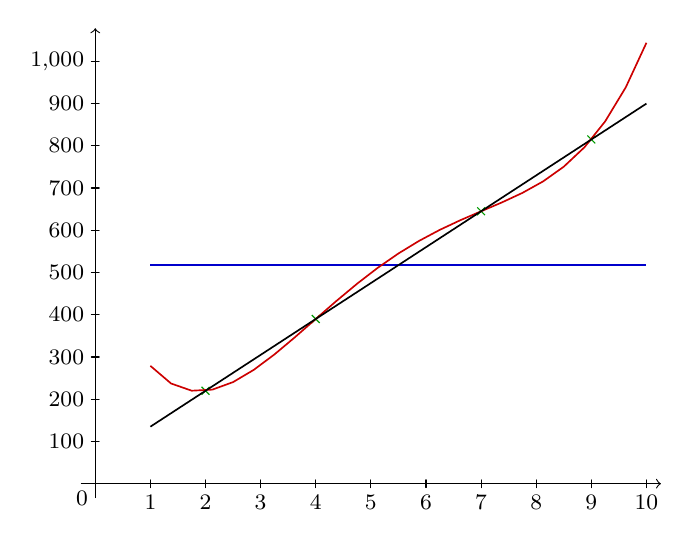
\begin{tikzpicture}[scale=.7]
\datavisualization[school book axes, 
visualize as line=lin,
visualize as line=poly,
visualize as line=mean,
visualize as scatter=data,
y axis={scaling = min at 0cm and max at 8cm,ticks={step=100}},
style sheet=strong colors
] 
data [set=lin,format=function] {
var x : interval [1:10];
func y = 85*(\value x)+50;
}
data [set=poly,format=function] {
var x : interval [1:10];
func y = 554 +(\value x)*(-421+167*(\value x)-22*(\value x)*(\value x)+(\value x)*(\value x)*(\value x));
}
data [set=mean,format=function] {
var x : interval [1:10];
func y = 517.5;
}
data[set=data]  {
x, y
2, (85*2+50)
4, (85*4+50)
7, (85*7+50)
9, (85*9+50)
}
;
\end{tikzpicture}
\end{center}
\end{frame}

\begin{frame}{Znajdźmy więcej prosiaków: zbiór testowy}
Czarne: $y=85x+50 \qquad MSE=0$ \\
Czerwone: $y=x^4-22x^3+167x^2-421x+554 \qquad MSE=7296$ \\
Niebieskie: $y=517{,}5 \qquad MSE=64423$

\begin{center}
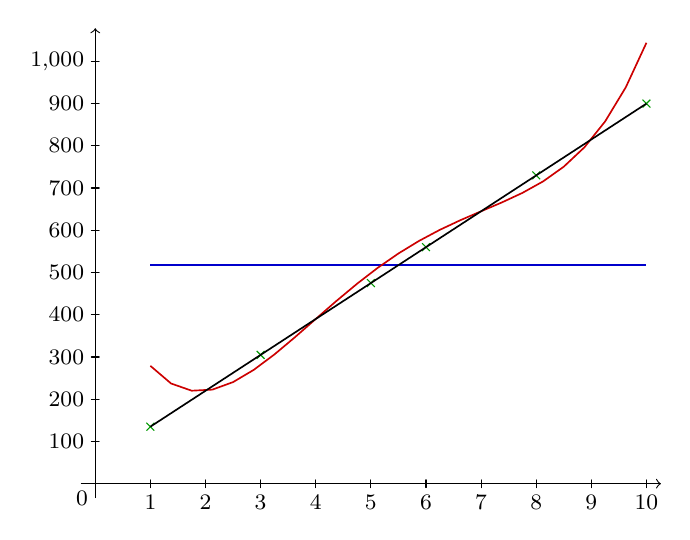
\begin{tikzpicture}[scale=.7]
\datavisualization[school book axes, 
visualize as line=lin,
visualize as line=poly,
visualize as line=mean,
visualize as scatter=data,
y axis={scaling = min at 0cm and max at 8cm,ticks={step=100}},
style sheet=strong colors
] 
data [set=lin,format=function] {
var x : interval [1:10];
func y = 85*(\value x)+50;
}
data [set=poly,format=function] {
var x : interval [1:10];
func y = 554 +(\value x)*(-421+167*(\value x)-22*(\value x)*(\value x)+(\value x)*(\value x)*(\value x));
}
data [set=mean,format=function] {
var x : interval [1:10];
func y = 517.5;
}
data[set=data,format=function]  {
var x : {1,3,5,6,8,10};
func y = 85*(\value x)+50;
}
;
\end{tikzpicture}
\end{center}
\end{frame}

\begin{frame}{Czy prosiaki uczące i prosiaki testowe się różnią?}
\begin{block}{Założenie i.i.d -- Identicially and idependently distributed}
Zakłada się, że wszystkie przykłady uczące i testowe pochodzą \alert{z tego samego rozkładu prawdopodobieństwa}, i zostały wybrane z niego \alert{niezależnie od siebie}.
\end{block}
\end{frame}

\begin{frame}{Zbyt słabe i nadmierne dopasowanie}
\begin{block}{Zbyt słabe dopasowanie \ang{underfitting}}
Duży błąd na zbiorze uczącym i duży błąd na zbiorze testowym
\end{block}
\vfill
\begin{block}{Nadmierne dopasowanie (przeuczenie) \ang{overfitting}}
Mały błąd na zbiorze uczącym i duży błąd na zbiorze testowym
\end{block}
\end{frame}

\begin{frame}{Zbyt słabe i nadmierne dopasowanie}
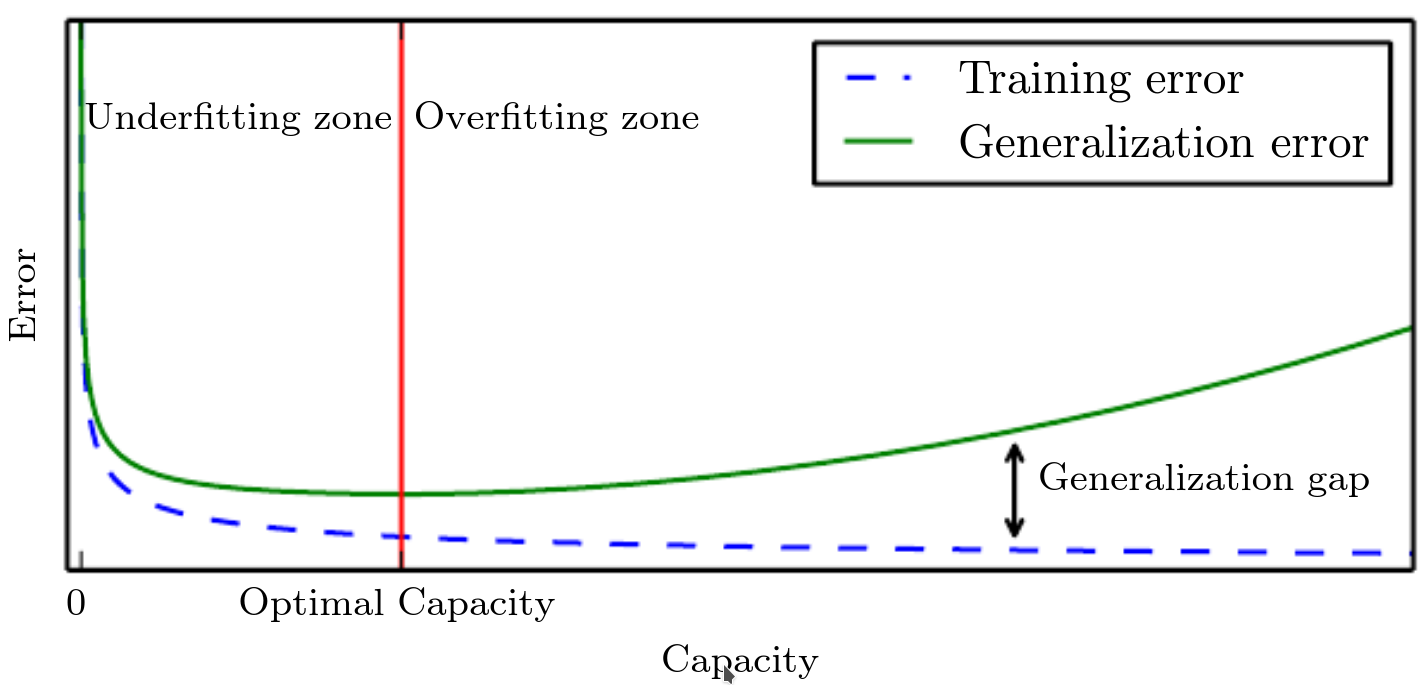
\includegraphics[width=\textwidth]{underfitting-overfitting.png}
\vfill
{\footnotesize I. Goodfellow, Y. Bengio, A. Courville \emph{Deep Learning} MIT Press 2016, str. 112}
\end{frame}

\begin{frame}{Parametry i hiperparametry}
\begin{description}
\item[parametry] są dobierane przez algorytm w procesie uczenia, np. wektor $\vec{w}$ w regresji liniowej
\item[hiperparametry] są dobierane przez użytkownika, żeby sterować procesem uczenia, np. stopień wielomianu w regresji wielomianowej
\end{description}
\end{frame}

\begin{frame}{Dobór hiperparametrów i zbiór walidujący}
\begin{block}{}
Dobór hiperparametrów za pomocą zbioru testowego prowadzi do przeuczenia
\end{block}

\pause
\vfill

\begin{itemize}
\item dobór \alert{parametrów} (uczenie) przez minimalizację błędu na zbiorze \alert{uczącym}
\item dobór \alert{hiperparametrów} przez minimalizację błędu na zbiorze \alert{walidującym}
\item szacowanie jakości na zbiorze \alert{testowym}
\end{itemize}
\end{frame}

\begin{frame}{Zwyczajowy podział danych}

Podział losowy w nastepujących proporcjach
\begin{description}
\item[zbiór testowy] $70\%$
\item[zbiór walidujący] $10\%$
\item[zbiór testowy] $20\%$
\end{description}
\end{frame}

\begin{frame}{Sprawdzian krzyżowy \ang{cross-validation}}
\begin{enumerate}
\item Zbiór uczący dzielony jest na $k$ podzbiorów
\item Dla $i=1,2,\ldots, k$:
\begin{description}
\item[zbiór walidujący] podzbiór $i$
\item[zbiór uczący]  wszystkie pozostałe podzbiory
\end{description}
\item Za wynik walidacji przyjmuje się średnią ze wszystkich $k$ walidacji (odchylenie standardowe gratis!)
\end{enumerate}

\vfill
Jakie są zalety i wady w stosunku do poprzedniego podejścia?
\end{frame}

\begin{frame}{Problemy z regresją liniową}
\[ \vec{w}={\underbrace{\left(\vec{X}^T\vec{X}\right)}_{p\times p}}^{-1}\vec{X}^T\vec{y} \]
\begin{itemize}
\item<+-> Złożoność odwracania macierzy: $O(p^{2.4})$ \\
\item<+-> Problemy numeryczne
\item<+-> Trudności z uogólnieniem: trzeba \alert{rozwiązać} równanie
\end{itemize}
\end{frame}

\end{document}